\documentclass[preprint,12pt,authoryear]{elsarticle}
\usepackage[T1]{fontenc}
\usepackage[utf8]{inputenc}
\usepackage{lmodern}
\usepackage{amsmath,amssymb}
\usepackage{booktabs,tabularx,array}
\usepackage{graphicx}
\usepackage{flafter}
\usepackage{placeins}
\usepackage{microtype}
\usepackage[hidelinks]{hyperref}
\renewcommand{\topfraction}{0.9}
\renewcommand{\bottomfraction}{0.8}
\renewcommand{\textfraction}{0.05}
\renewcommand{\floatpagefraction}{0.8}
\setlength{\emergencystretch}{2em}
\journal{Data \& Knowledge Engineering}
\begin{document}
\begin{frontmatter}
\title{History-Sensitive Admission of Corrected Records}
\begin{abstract}
Authoritative records can have identical final values yet arise from different proposal and authorization histories. We study correction-aware admission as a relation linking an exact persisted candidate, an attributable authorization of an explicit value, and a complete successor whose every field has a source. The relation preserves the proposal when a reviewer authorizes a correction. Within a declared observation model, five paired histories identify information classes that distinguish candidate substitution, correction misattribution, stale authorization, fragmented successors, and source ambiguity. We encode the relation in Alloy and implement it in a transactional SQLite service. An independently written event journal with exact candidate binding agreed with the service on all 165 paired constructed cases and their provenance-query answers; a rich-context journal without that binding admitted 15 equal-valued candidate substitutions and produced ambiguous reviewed-candidate answers. Formal–concrete checks and a fault catalogue test the persisted realization. A browser experiment locates the review-to-confirmation boundary, while current-version measurements characterize admission and trace costs. These results provide a checkable basis for admitting corrected records across the evaluated storage designs.

\end{abstract}
\end{frontmatter}

\section{Introduction}

A stored field value answers \emph{what the record says now}. It does not, by itself, answer which proposal was reviewed or which value the reviewer authorized. Suppose a record has quantity 90, a candidate proposes 100, and a reviewer authorizes a correction to 101. The resulting quantity is 101. The same value could follow from accepting a candidate that originally proposed 101. These histories assign different roles to the proposer and reviewer, even though their current values agree.

Candidate identity introduces a sharper test. Let two persisted candidates propose 100 for the same field under the retained review context. A reviewer inspects candidate $c_1$ and authorizes 101, but candidate $c_2$ is supplied for admission. A value-level check can observe the approved value 101 and the committed value 101 without identifying the substitution. The question is whether the authorization applies to the particular candidate that became part of the record's history (Fig.~\ref{fig:1}).

\begin{figure}[!htbp]
\centering
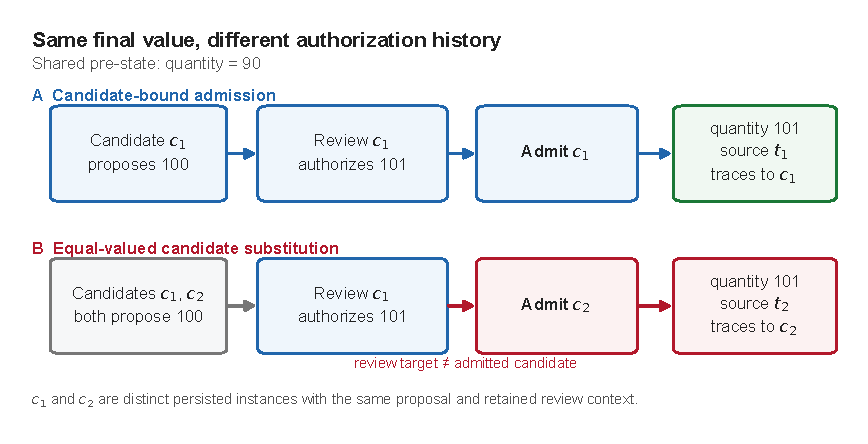
\includegraphics[width=\linewidth]{figures/fig1_same_value_different_history.pdf}
\caption{A constructed equal-valued candidate substitution. Both paths start at quantity 90 and commit 101. In path A, authorization targets the candidate admitted by the transaction. In path B, a context-only control admits $c_2$ after authorization targeted a distinct, equal-valued $c_1$; candidate-bound admission rejects this substitution. The field source is a transition ($t_1$ or $t_2$), from which the admitted candidate is traced. OpenAI Codex (GPT-6, accessed 24 September 2026) assisted with the layout and Matplotlib 3.10.8 vector-rendering code; the candidate, authorization, and source links were checked against the admission relation.}
\label{fig:1}
\end{figure}

Provenance can explain how data was derived or updated. Content-based approval can hold an update for review. Our question is narrower: \textbf{which persisted proposal, explicit authorized value, and field sources must be linked when a corrected record becomes authoritative?} This is an admission relation, rather than a new transaction or provenance primitive.

We model that relationship among a pre-state, candidate, authorization, and successor state. The candidate retains its proposal, evidence, field, record, and expected version. The authorization identifies the candidate instance, the reviewer, and the value permitted to enter the record. A correction may therefore commit a value different from the proposal without rewriting what was proposed. One transaction creates the successor and its total field-source map. Changed fields point to new transitions; unchanged fields keep their exact prior sources. The relationship is defined over these semantic roles, so it can be realized through different storage structures.

The model also explains what an admission decision must distinguish. Five paired histories isolate candidate context, value roles, freshness, successor completeness, and field sources. Within the declared observation model, each pair becomes indistinguishable when its corresponding information class is omitted. The equal-valued candidate case then asks a further question: can the review identify one persisted instance when all retained contextual values agree?

Rich review context offers a useful test of the contribution. It may retain field, version, evidence, and review details while omitting an explicit identifier for the reviewed candidate. We implement that design in a study-specific event journal and compare it with an otherwise matching journal that records exact candidate binding and with a transactional reference service. In the constructed comparison, the exactly bound journal and reference service agree on all 165 paired cases and their provenance-query answers. The context-only journal admits 15 equal-valued substitutions and leaves reviewed-candidate answers ambiguous. The result locates the distinguishing condition in the authorization relation rather than in the choice of event logging or relational tables.

The formal and persisted checks address whether this decision can be enforced beyond the motivating example. Bounded Alloy analysis tests the encoded relation; formal–concrete projections and a 35-case fault catalogue test its transactional realization and reverse trace.

Review occurs before that service is called, so we also examine how the intended decision reaches it. In scripted browser cases, a server-held review-session binding rejects request substitutions that the original confirmation path accepts from its caller. Display-only substitution remains visible to the independent observer. The two outcomes identify separate responsibilities for review presentation and transactional admission. Finally, current-version admission, trace, and storage measurements characterize the cost of enforcing and querying the recorded relationships.

The contribution is a correction-aware admission relation and a conditional characterization of five failure-distinguishing information classes. The implementations and experiments test the relation across two storage designs and at the review boundary. The organizing link runs from the \textbf{candidate reviewed}, through the \textbf{value authorized}, to the \textbf{complete successor committed}.

\section{Related work and position}

Query provenance distinguishes why an answer exists and where its data originated (\citet{buneman2001why}). Provenance for curated databases records manual copying and attribution (\citet{buneman2006curated}). Transaction reenactment reconstructs the provenance of updates from database history (\citet{arab2018reenactment}). The PROV data model~\citep{w3c2013prov} provides general entities, activities, and agents. These accounts motivate retaining history and sources; our relation fixes the conditions under which a reviewed correction creates the next authoritative version.

Content-based update authorization is also established: bdbms~\citep{eltabakh2006bdbms} allows curators to approve or disapprove pending updates based on their content. We build on that idea. The distinction tested here is between authorizing a value in retained context and authorizing that value \emph{for one persisted candidate instance}. The equal-valued substitution case exposes the difference even when field, version, evidence, and final value agree. Complete successor construction and per-field source links make the resulting decision queryable after admission.

\section{Admission semantics for corrected records}

\subsection{Proposal, authorization, and authority}

Let $r$ denote a record with authoritative fields $F_r$. Its version $v$ has a value map $V_v$ and a source map $P_v$, both defined for every field in $F_r$. The source of a field identifies a persisted transition that explains its current value. A candidate $c$ is a persisted proposal for one record and field. It retains evidence identity, a proposed value $x_c$, the expected record version, a producer, and an identity that distinguishes it from other candidate instances. Evidence identity combines content with its canonical record- and field-related locator; equal-looking content at a different location need not denote the same evidence instance.

An authorization $a$ records a reviewer, the exact candidate reviewed, and an explicit authorized value $x_a$. When $x_a=x_c$, the decision accepts the proposal. When $x_a\ne x_c$, it corrects it. Both decisions leave the candidate's proposal intact. The committed field takes $x_a$; a later query can still return $x_c$ and identify the reviewer who permitted the difference. Values are compared by canonical JSON representation so that a numeric or Boolean type change is not silently treated as an unchanged field.

For a single changed field, admission is the state relation

\[
\operatorname{Admit}(S_v,c,a)=S_{v+1},
\qquad S_v=(V_v,P_v).
\]
The relation holds when the authorization names the persisted candidate and explicit value; the candidate's record, field, evidence, and expected version match the attempted update; the reviewer passes the applicable policy check; and the successor is complete. A stale candidate cannot authorize an update to a later pre-state. If any check fails, the attempted admission leaves authoritative state unchanged.

\subsection{A complete successor and its source map}

For a multi-field attempt, let $U$ be its submitted items and $B\subseteq U$ the admitted items. All items in $B$ share one record, reviewer principal, current pre-version, and successor; each addresses a distinct field and has a candidate-bound authorization. A post-initial concrete admission selects items whose authorized values change their fields. It creates one successor in one transaction, with $\{i.f\mid i\in B\}=\Delta(V_v,V_{v+1})$ and exactly one transition per admitted item. Unchanged submitted items keep their prior values and exact sources; they create no transition or authorization binding. The first certificate-era version instead covers every field. The Alloy model permits a historical same-value admission for correspondence with its singleton model, so the changed-field equality here describes the post-initial concrete path.

For every changed field $f$, $V_{v+1}(f)$ is the authorized value and $P_{v+1}(f)$ is its new transition. For every unchanged field $g$,

\[
V_{v+1}(g)=V_v(g),\qquad P_{v+1}(g)=P_v(g).
\]
This copy-forward rule matters even when an update changes only one field: the resulting record remains a complete version with an exact source for every field. Reverse tracing follows a field's transition to its authorization, candidate, evidence and producer. The trace distinguishes the value proposed from the value authorized and identifies the version in which the value entered the record (Fig.~\ref{fig:2}).

\begin{figure}[!htbp]
\centering
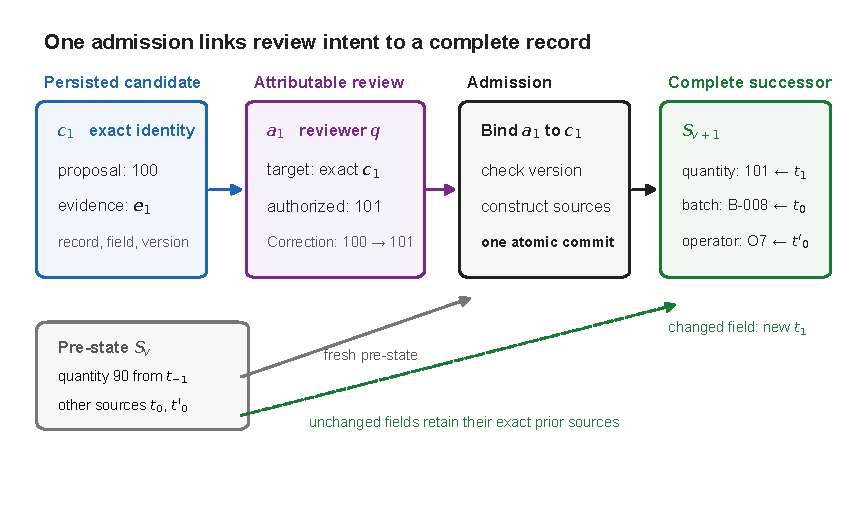
\includegraphics[width=\linewidth]{figures/fig2_admission_relation.pdf}
\caption{The correction-aware admission relation. The persisted candidate proposes 100; the reviewer authorizes 101 for that candidate. The transaction checks the binding and current pre-state before creating one successor. The changed quantity obtains a new source transition, while unchanged fields retain their prior source transitions. OpenAI Codex (GPT-6, accessed 24 September 2026) assisted with the diagram layout and Matplotlib 3.10.8 vector-rendering code; the value roles, transaction edge, and field-source arrows were checked against the stated relation.}
\label{fig:2}
\end{figure}

\subsection{What the relation makes queryable}

The resulting data model supports two complementary queries. An admission query asks whether a proposed transition has a candidate-bound authorization for the value it would write to the current version. A provenance query starts from a committed field and returns its source transition, the candidate behind it, the candidate's original proposal, the authorized value, and the responsible reviewer. Both queries operate on the same persisted relationships. This avoids relying on the final value alone to reconstruct a decision that may have involved correction or candidate substitution.

\section{Failure distinguishability}

\subsection{Histories and observations}

A history contains candidate persistence, review and authorization, admission attempts, commits or unchanged state, and later trace queries. Let $O(h)$ denote its authority outcome: whether the update is admissible and whether the resulting version and trace are complete. Let $\pi_I(h)$ retain only information in observation classes $I$. This separates an outcome from what a restricted observer can see. The five classes each support a distinct admission question (Table~\ref{tab:1}).

\begin{table}[tbp]
\caption{Five failure-distinguishing information classes in the declared history and observation model. A class describes information required for the stated comparison; several classes may share one physical representation.}
\label{tab:1}
\centering
\footnotesize
\begin{tabularx}{\linewidth}{@{}>{\raggedright\arraybackslash}p{0.23\linewidth}>{\raggedright\arraybackslash}X>{\raggedright\arraybackslash}X@{}}
\toprule
Class & Information retained & Histories separated \\
\midrule
Candidate identity and context ($D_C$) & Exact candidate plus record, field, evidence, and producer context & Authorized candidate versus an equal-valued substitute \\
Value roles ($D_V$) & Proposal, authorized value, committed value, and their roles & Preserved correction versus erased or false attribution \\
Freshness ($D_F$) & Expected and transactionally observed pre-state & Current approval versus approval after supersession \\
Successor completeness ($D_B$) & Declared effects, actual commit grouping, and successor count & One atomic batch versus fragmented updates with the same endpoint \\
Field sources ($D_S$) & A total field-to-transition map and exact copy-forward links & Complete trace versus missing or conflicting source \\
\bottomrule
\end{tabularx}
\end{table}

\textbf{Proposition 1 (conditional failure distinguishability).} Let $\mathcal D=\{D_C,D_V,D_F,D_B,D_S\}$ be the declared observation classes. For every $d\in\mathcal D$, the declared failure model contains histories $h_d^+$ and $h_d^-$ such that $O(h_d^+)\ne O(h_d^-)$ and $\pi_{\mathcal D\setminus\{d\}}(h_d^+)=\pi_{\mathcal D\setminus\{d\}}(h_d^-)$. Hence a decision based only on the other four classes cannot distinguish that paired failure family within this model.

The five witnesses establish the proposition by construction. For $D_C$, the admitted equal-valued candidate changes its non-temporal context. For $D_V$, the candidate and final value stay fixed but the correction is attributed to the producer instead of the reviewer. For $D_F$, a version is superseded between authorization and admission. For $D_B$, one atomic batch and two fragmented commits reach the same endpoint but differ in their intermediate state. For $D_S$, one successor field loses its source anchor. An additional identity-isolation pair fixes two candidates' retained review context and changes only which instance is admitted. This pair tests exact binding within the broader $D_C$ class; it does not assert a sixth universally necessary class.

\subsection{From distinctions to enforceable conditions}

The five pairs organize the admission checks. Candidate identity and value roles bind review to the proposed artifact and the value actually authorized. Freshness connects that decision to the current pre-state. Successor completeness prevents a batch from installing only some of its effects. Field-source totality ensures that a successful version can be traced for both changed and unchanged fields. This analysis motivates a joint integrity relation: a transaction can be atomic yet have the wrong review target, or preserve the right value while losing the source needed to explain it.

We encode the relation in Alloy to test legal constructions, malformed attempts, and preservation properties in finite scopes. Separate omission witnesses establish the information-class result, while conjunct-removal checks test the sensitivity of particular relational encodings. The two checks serve different purposes: one concerns what an observer can distinguish; the other concerns what a specified admission predicate accepts.

\section{Two storage realizations and the review boundary}

\subsection{Transactional reference service}

The reference realization stores immutable candidates and evidence references alongside decisions, authorization bindings, record versions, transitions, and field-source links. At confirmation, it validates the selected candidate and authorized value, rechecks reviewer policy and the current record version, then builds the complete successor. A compare-and-swap on the version protects the admission attempt. Decision, transitions, version, sources, and audit effects are written in one database transaction; a rejected attempt does not install a partial authoritative version.

A reverse-trace operation starts at a committed field and resolves its source through the admission records. It checks the candidate, authorization, evidence, and value relationships on the path. This makes the trace an integrity-bearing query over persisted objects rather than a textual explanation reconstructed from the final field value.

\subsection{Event-journal comparison}

To test whether the relation depends on the reference schema, we implement a separate SQLite event journal for the study. It retains candidate records, rich review context, version checks, immutable events, complete field-source maps, and transactional updates. Two configurations differ in one policy-relevant observation: the context-only journal retains the reviewed field, version, evidence, and context but omits the exact reviewed-candidate identity from its authorization check; the exact journal retains that identity. Both implement the same tested value, freshness, and source requirements.

This comparison isolates candidate-instance binding within a strong recorded context. It also gives a constructive alternative implementation: an event journal can enforce the evaluated admission relation once the exact binding is represented and checked. The comparison concerns the shared tested contract and workloads, not feature-by-feature equivalence of the surrounding applications.

\subsection{Transferring review intent to confirmation}

The database can check an authorization only after the review interface has formed it. The reference confirmation path receives candidate, reviewer, and authorized value from a trusted caller. We therefore add an experimental server-held review session that records the reviewed target and permitted value before confirmation, then checks the request against that session. This lets us distinguish a request changed after review from a display changed without altering the server-held target. These are different boundaries: the former concerns transmission of review intent; the latter concerns what the reviewer was shown.

\section{Evaluation design}

We organize the evaluation around three questions: whether the specified relation is reflected in persisted behavior, whether exact candidate binding changes decisions and provenance answers under rich-context controls, and what happens at the review and query boundaries. Complete configurations and raw records are deposited with the artifact; the main text reports the comparisons needed to interpret the claims.

\subsection{Formal and persisted-state checks}

Two finite Alloy profiles exercise legal admissions, selected constraint removals, source corruption, and preservation assertions. A test-side projection independently reads selected pre- and post-states from SQLite and maps them to fixed relational instances. Its intended cases cover singleton and batch admissions, correction, copy-forward, staleness, and whole-batch rejection. A separate 35-case catalogue tests the production-facing service with legal histories, rejection, rollback, stateful evolution, schema prevention, corruption diagnosis, and oracle sensitivity. Rejected attempts are checked against a complete logical database digest; corruption cases require a trace or independent-oracle diagnosis.

\subsection{Cross-implementation cases and provenance queries}

The event-journal comparison uses 15 inputs across 11 constructed case families and three mechanisms: context-only journal, exact-binding journal, and the reference service. Twelve inputs are deterministically selected archived proposal values; three additional inputs probe JSON type boundaries. The archived cells contain four distinct proposal values. Cases cover acceptance, correction, multi-field updates, candidate and evidence substitutions, stale and replayed decisions, unauthorized values, and interrupted transactions. After each successful admission, an independent oracle asks field-level questions about proposal, authorized value, reviewer, reviewed candidate, current value, and source version.

The context-only policy still compares field, version, evidence, and retained review context. Its only intended relaxation is candidate-instance identity. We score value-level agreement and instance-level authorization separately so that rejecting an equal-valued replacement is not conflated with rejecting an incorrect final value.

\subsection{Browser and cost studies}

The review-boundary study runs three JSON value types through ten scripted interaction cases on each of two confirmation paths. An independent browser driver records the candidate and value displayed before review and compares them with the request and persisted result. Cases include legitimate acceptance, correction, reselection, request substitutions, stale and replayed submissions, rollback, and display-only substitution.

Current-version cost measurements use fixed admission and trace workloads. Complete confirmation is compared between the reference and exact journal under the shared tested workload; a separate prevalidated materialization comparison isolates a narrower persistence path. A 36-cell trace study holds the verifier fixed while changing three repository reads from bulk retrieval to identifier enumeration and point lookups. Every paired trace must return the same complete object. Synthetic storage fixtures characterize schema footprint at three transition counts. Figure generation reads the deposited summary tables; full observations and reproduction details remain in the supplement.

\section{Results}

\subsection{Exact binding separates equal-valued candidate instances}

All 495 cross-implementation executions completed: 15 inputs, 11 case families, and three mechanisms. The exact journal and reference service agreed on all 165 paired cases and their 810 field-level provenance answers per mechanism. Each admitted 45 legal cases and rejected 120 without fact writes. The context-only journal also admitted the legal cases, but accepted 15 equal-valued candidate substitutions. Those cases satisfy its value-and-context policy while violating instance-level authorization. Of 1,080 context-only field-level answers, 60 reviewed-candidate answers were ambiguous; the two exactly bound mechanisms produced no ambiguity (Fig.~\ref{fig:3}). Under a value-only policy, the 15 rejected substitutions count as false rejections for the exact journal and reference service. Under the stated instance-level relation, they are required rejections.

\begin{figure}[!htbp]
\centering
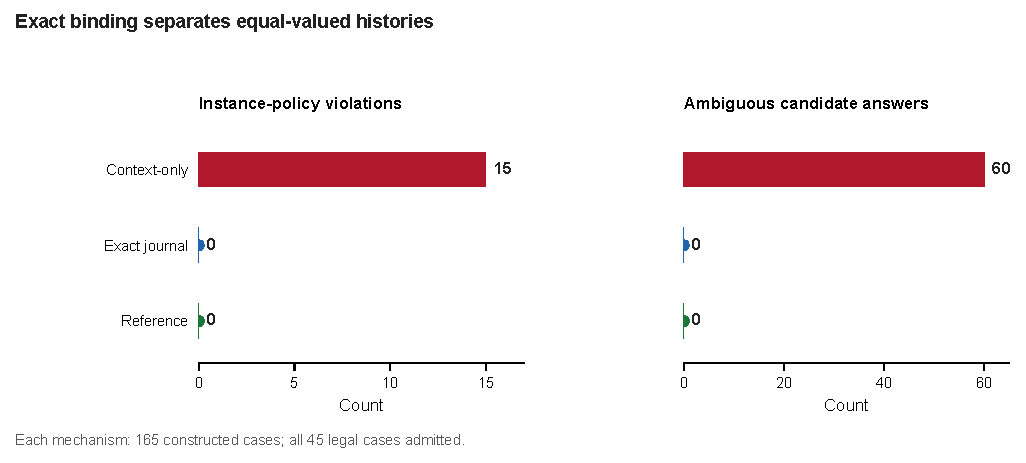
\includegraphics[width=\linewidth]{figures/fig3_candidate_binding_comparison.pdf}
\caption{Instance-policy violations and ambiguous reviewed-candidate answers across the three mechanisms. Each mechanism completed 165 constructed cases and admitted all 45 legal cases. Ambiguous answers are field-level query answers, not additional admission cases. The plot was generated from the deposited comparison summary by a reproducible Matplotlib 3.10.8 script assisted by OpenAI Codex (GPT-6, accessed 24 September 2026); the plotted counts were checked against the source table.}
\label{fig:3}
\end{figure}

Rich context narrows which candidates are compatible with a review, but equal-valued instances can remain equivalent under the context-only policy. Recording the reviewed instance resolves both the admission decision and the later query. The result identifies a relation that the tested event journal and reference service can both enforce.

\subsection{The relation survives bounded and persisted checks}

Both Alloy profiles produced the declared legal, malformed, and source-corrupt witness classes. Across the two profiles, all 72 command outcomes matched the manifest. Each selected conjunct removal admitted a paired malformed history that the full relation rejected, while the checked preservation assertions found no counterexample within their finite scopes. The independent database projection accepted nine intended cases and rejected twenty mapping mutants. All 35 declared production-facing catalogue cases passed their specified admission, rejection, or diagnosis criteria. Together, these results link the admission predicate to the stored version and its trace; the paired-history construction supplies the separate observation-level argument.

\subsection{Review intent has a distinct transfer boundary}

Across 60 scripted browser cases, each path admitted all nine legitimate controls. The original confirmation path accepted nine request substitutions inconsistent with the review intent recorded by the browser driver; the server-held session gate rejected all nine. Both paths rejected stale submissions, replays, and precommit interruptions without fact writes. Three display-only substitutions on each path left the server-held target unchanged while changing what appeared in the browser; both paths admitted them (Table~\ref{tab:2}).

\begin{table}[tbp]
\caption{Scripted review-boundary outcomes across three input types. The original path treats its caller's confirmation parameters as the review decision; the experimental session gate checks them against server-held review intent. Display-only substitution probes a different, presentation-side relationship.}
\label{tab:2}
\centering
\footnotesize
\begin{tabular}{@{}>{\raggedright\arraybackslash}p{0.21\linewidth}*{4}{>{\centering\arraybackslash}p{0.165\linewidth}}@{}}
\toprule
Confirmation path & Legitimate controls admitted & Request substitutions admitted & Display-only mismatches admitted & Rejected cases with fact writes \\
\midrule
Original confirmation & 9/9 & 9 & 3 & 0 \\
Server-held review session & 9/9 & 0 & 3 & 0 \\
\bottomrule
\end{tabular}
\end{table}

The session gate makes request-to-review consistency enforceable. The display-only controls locate the further requirement for a faithful review presentation: a server-side authorization link cannot describe what a reviewer saw if the display itself has changed independently.

\subsection{Admission and provenance-query costs}

The current-version study retained 22,400 measured admission and trace observations. Across the ten complete-confirmation cells, the reference implementation's median latency ranged from 28.79 to 712.00 ms; the exact journal ranged from 10.40 to 23.89 ms. These figures describe the two complete implementation paths under the stated call boundary. The separate prevalidated materialization study reports persistence costs after validation and planning; it is not used as a substitute for complete confirmation.

For tracing, all 36 cells returned identical complete objects under bulk and point-lookup access (Fig.~\ref{fig:4}). Bulk retrieval had a lower median latency in each paired cell. At 128 fields, 100 versions, and 1,000 records, its median was 170.24 ms, compared with 509.09 ms for point lookups; the corresponding SQL counts were 12 and 693. The contrast holds the verifier fixed and changes the repository access pattern. Storage fixtures show the footprint of complete authority and source relations over 1,000 to 100,000 transitions; the full cell table and measured database sizes are retained with the artifact.

\begin{figure}[!htbp]
\centering
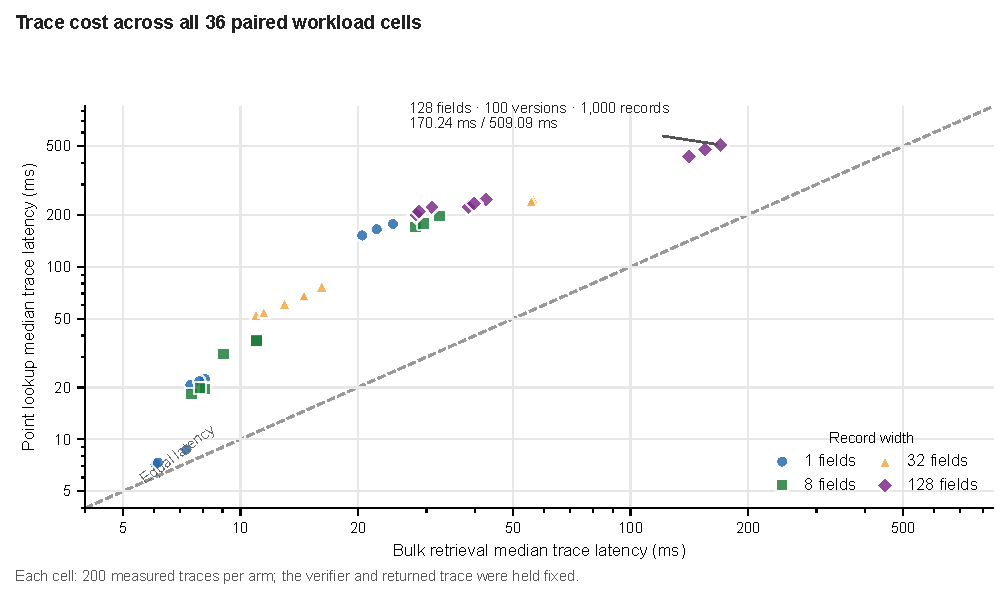
\includegraphics[width=\linewidth]{figures/fig4_trace_cost.pdf}
\caption{Median trace latency under two repository access patterns across all 36 paired cells. Each point represents 200 measured traces per arm; marker shape and color identify record width. The dashed line marks equal latency. The verifier and returned trace object are held fixed. The plot was generated from the deposited trace summary by a reproducible Matplotlib 3.10.8 script assisted by OpenAI Codex (GPT-6, accessed 24 September 2026); all 36 source pairs were included and checked.}
\label{fig:4}
\end{figure}

\FloatBarrier
\section{Data and knowledge engineering implications}

The experiments support a data-modeling interpretation of authorization. A review event carries authority for a particular candidate and explicit value; a fact transition records what was committed; and the successor's source map preserves the relation between current values and their origins. A provenance query can then recover both the proposal and the correction from the committed record. Treating these as separate but linked objects also makes equal-valued candidate substitution visible to an admission decision.

The event-journal result is useful because it shows that the integrity relation is portable across the evaluated storage structures. The choice of relational version tables or an immutable event journal affects engineering cost and query implementation, while the candidate-to-authorization link determines the tested instance-level decision. The browser result identifies where that link must be formed: the review process must establish the intended target before a transaction can enforce it.

The observation result applies to the declared history model; the implementation results apply to the evaluated service, journals, and workloads. Host authentication and the integrity of what a reviewer is shown remain external to the admission relation. At commit and during later tracing, the candidate, authorized value, and field sources remain explicitly linked.

\section{Conclusion}

Corrected records require more than an approved final value. We defined an admission relation that preserves the exact candidate reviewed, the separately authorized value, and a complete successor with per-field sources. Paired histories identify five distinctions that this relation must retain under the declared model. Formal checks, persisted-state tests, and a cross-implementation comparison connect the relation to executable behavior; browser and cost studies locate its interaction boundary and operational expense. The result is a concrete basis for making reviewed updates into attributable authoritative facts.

\section*{Artifact availability}

The \href{https://github.com/lhh666-6/auto-dete}{public artifact} contains the frozen reference implementation and formal materials. The \href{https://github.com/lhh666-6/auto-dete/tree/main/DKE-supplement}{DKE supplementary deposit} contains the event-journal comparison, browser study, current-version cost data, raw observations, and reproduction instructions.

\section*{Declaration of generative AI and AI-assisted technologies in manuscript preparation}

OpenAI Codex (GPT-6, accessed September 2026) assisted with organization and English drafting, with the layout and code for explanatory diagrams, and with reproducible plotting code for data figures. The explanatory diagrams were rendered with Matplotlib 3.10.8 and checked against the specified admission relationships. Data figures, where included, are generated from deposited tables without altering the underlying observations. The authors retain responsibility for reviewing, editing, and approving the final manuscript and figures.

\bibliographystyle{elsarticle-harv}
\bibliography{references}
\end{document}
